\section{Approach}
\subsection{Simulated Network}

The network of our simulation is designed to give a real-time nature to the data transfer 
between the Tennessee Eastman(TE) physical simulation and the TE Controller. 
Both the controller and simulation are written in Matlab and connected to our network with 
the OMNeTBridge Class. (These are described in later sections.)

The network is based primarily on two factory level components, sensors and actuators, that 
send data to a remote facility that sends back control signals. This is based on most SCADA 
systems that need remote facilities to monitor their data. These signals are sent over a 
simulated "Internet" that allows accurate packet loss, bit errors and data rates. 

Due to limitations of the default Inet packets we are not actually sending the data through 
the network. Rather, the packets the controller receives act as a trigger to have the 
controller update the data from that sensor, and send an update to the actuators if need be. 

\subsection{Matlab Simulation}
We chose to use MATLAB simulation for the physical system and it's controls, as there are 
many chemical process models currently implemented in MATLAB. This allows for the ease of 
swapping out current MATLAB models for new ones.

\subsubsection{Tennessee Eastman}
 In order to keep the complexity down, we decided to model the chemical process in the plant 
 as a simplified Tennessee Eastman problem\citation{Ricker}. Due to this approach, we looked 
 to previous work in the field, and found many models already modeled in a hybrid of FORTRAN 
 and MATLAB.  However, this introduced more complexity, due to using three different 
 programming languages to implement what should be simpler.  Therefore, we would build a 
 custom MATLAB class that contained the same functionality.  This includes a both the 
 simulation of the actual Tennessee Eastman system, and the steady state controller 
 calculations.


\subsection{C++ to Matlab Bridge}



\begin{figure*}
        \centering
		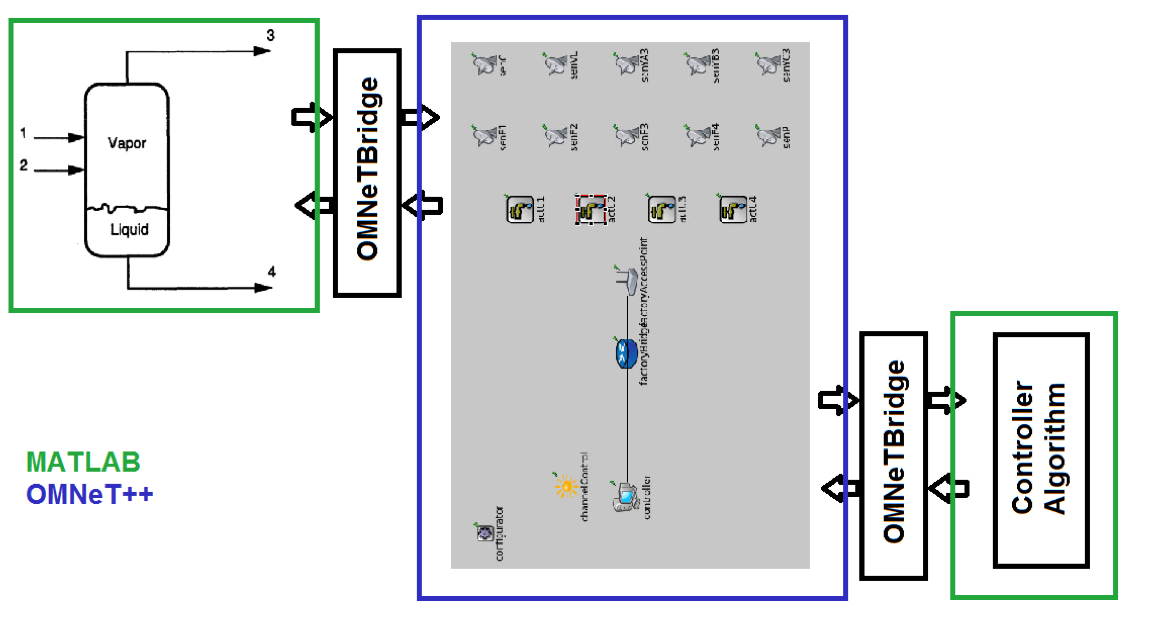
\includegraphics[width=0.8\textwidth]{figs/system.png}
        \caption{System Diagram.}
        \label{fig:system}        
\end{figure*}
